This section looks at previous work in similar fields. It starts with presenting the paper that offer the idea that this thesis further explores, and then looks at past research on using Twitter and critical infrastructure data for similar tasks.

\section{Spatiotemporal information from urban systems}
In the novel study of "Detecting flu outbreaks based on spatiotemporal information from an urban system", which is the base idea for this thesis, Grottenberg et al. \cite{spatiotemp_urban_sys} outlines a design for a system for surveillance of flu outbreaks. Emphasis on the belief that real-time data flows could prove useful in both understanding social functions during disasters and crisis as well as give " ... actionable intelligence for use in influenza management efforts.". The goal would be to extend the already implemented infrastructure with an approach to monitor human behaviour in trends throughout the influenza activity in hope for discrepancies detected through spatial analysis on important measurements. The borrowed figure \ref{fig:grottenberg} from his article sums up what this thesis hopes to accomplish, namely to find a correlation between different datasets and the datasets from the Norwegian public health institution (NIPH), this interference of public behaviour would become visible in essential criterion.
This short read \cite{spatiotemp_urban_sys} is recommended as it gives a more in-depth understanding of the incentive for this thesis.

\begin{figure}[h]
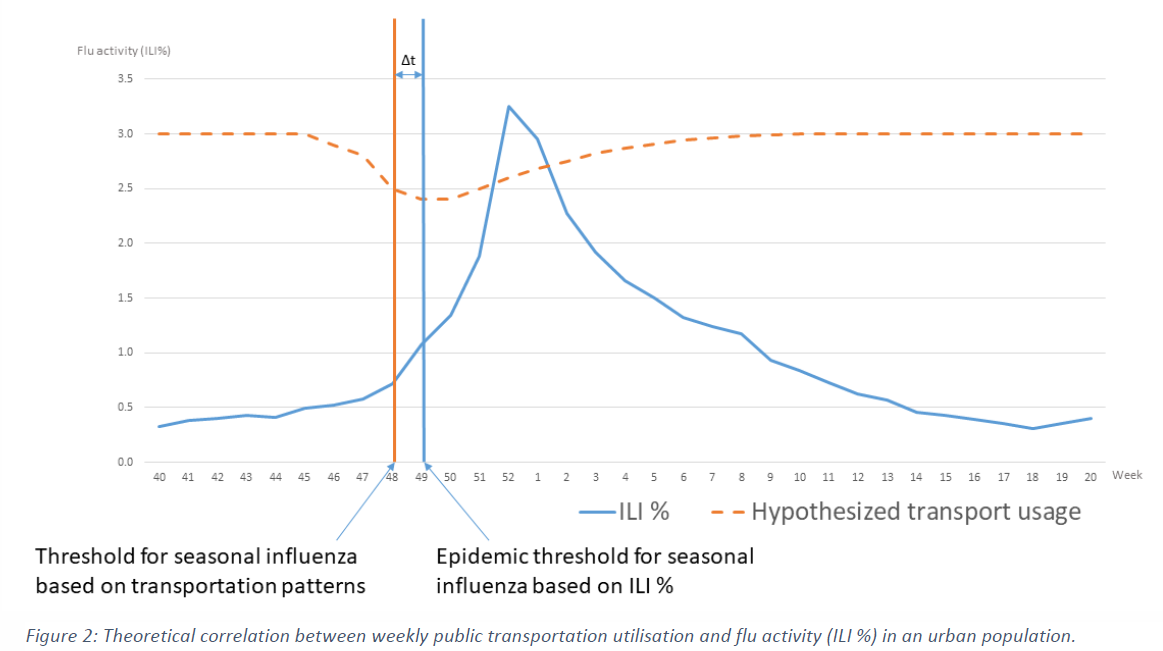
\includegraphics[width=16cm]{grottenberg}
\centering
\caption{Figure from Grottenberg et al. \cite{spatiotemp_urban_sys}}
\label{fig:grottenberg}
\end{figure}


\section{Spatiotemporal information from VGI}
Volunteered Geographic Information (VGI) is peer-produced crowd spatial data for use in crisis responses. Mobilizing digital volunteers to help with disastrous events alleviates the data needed by relief agents, VGI is peer-produced spatial data that is highly up-to-date. In 2010 the Haiti Earthquake levelled many official government buildings and with them access to official mapping resources\cite{palen2015success}. In just a few days volunteers contributed to OpenStreetMap\cite{OpenStreetMap} (OSM) and created an even better map of Haiti using satellite images by individually identifying map resources. A similar approach was initiated during the 2015 Nepal earthquake\cite{hu2016task}. Anderson et al\cite{anderson2018crowd} describes methods for evaluating the quality of VGI and to the development of "... rapid metrics of quality for digital data generated under socially distributed conditions ...". They reason that peer production platforms will be a more integrated part of disaster management and that when the risk of lives and infrastructure is present a solid basis for quality control of VGI information should be established.

\section{Data management and critical infrastructure}
This thesis touches upon data management and development of crisis response systems. The proposed system would act as a tool in a larger system in the development of support decision making in the event of an epidemic influenza preparedness and outbreak. 

Responding to extensive crisis or disasters requires coordination between a multitude of relief agencies, and this demands the right information at the right time. A system that can detect an emergence of a possible influenza outbreak would be an aiding factor to this. Gonzales et al. \cite{gonzalez2009framework} goes into general details of how the quality of information during a crisis response is important and how to better coordinate relief agencies with the right information at the right time. Their report includes a case study where simulation of interagency crisis response by the port of Rotterdam in the Netherlands, in particular this case study emphasise the qualitative trial and strategy throughout interagency crisis management. Extensive emergencies requires involvement of a multitude of relief and other regional service assets to cooperate and share relevant and timely information. The specifics of the case study simulates the collision of a containership with a passenger ship where the containership explodes and leaks hazardous chemicals. Responding to such a catastrophic tense event requires cooperation of multiple authorities from professional representatives guided by regional and port experts. Gonzales et al. concludes that designing a computer based system for management and automation services of a work flow information conductor would better the over all quality of response and guidance. The system proposed by this thesis could be a module of such a system. 

Machine-learning algorithms may also be of use in spatiotemporal analysis of social media data for disasters and damage assessment. Resch et al \cite{resch2018combining} explains how the current management of disasters have several shortcomings that can be solved by machine-learning topic models and spatiotemporal analysis. Temporal lags and limited resolution of information prevents successful and accurate resource deployment, advantages of new approaches with real-time collecting of data, like social media and other crowdsourcing networks "can significantly improve disaster management". Resch et al proposes a new approach to analyse social media with the combination of semantic machine-learning algorithms with spatio and temporal analysis. The challenge is detecting data flow continuously without prior analysis and knowledge about the event in question. Their results show remarkable improvement to accurate event tracking and other hotspots, disaster management and valuable insight to affected regions and assets.

Simulation modules could also be added to this system. This thesis is not a simulation tool but it is worth mentioning that there are several such proposed models of influenza and other disease simulation implementations. Shao et al. \cite{shao2016forecasting} ask the question of whether it is possible by monitoring public urban data by designing a social network sensor for epidemics to predict the coming outline of an overall epidemic, and simulates this. Developing sufficient heuristics in order to adpot social sensors to forecast influenza outbreaks when probabilistic views of structure of simulated influenza propagations interests public health dignitaries and govermental stratagem designers. There are many more simulation tools, another is proposed by Stein et al. \cite{stein2012development} which models an influenza outbreak in two provinces of Lao. Stein et al's framework proposes that planning for influenza outbreaks is an exigent engagement that requires predictive models to better evaluate responsive strategies. Stein et al freely offers their simulation too called AsianFluCap on their website and describes it as ".. a user-friendly, comprehensive and flexible simulation tool which can be used by decision makers involved in pandemic preparedness to estimate and compare the impact on health care resource capacity during different pandemic scenarios.". Simulations are a way of preparing and training in order to reveal flaws and evaluation of response plans and deployment of limited health care resources, and raise awareness of surges in sudden resource demands during pandemics, especially so where such resources are scarce and efficient delegation is important.

\section{The Ebola epidemic}
The west African Ebola viral haemorrhagic fever (VHF) epidemic lasted from 2013 to 2016 and spread to a wide part of the globe. Ebola causes fever, sore throat, muscular pain, headaches and lastly internal haemorrhage (internal bleeding), the death rate is about 25\% to 95\% with an average of 50\%\cite{who_ebola}. 
Tom Koch\cite{koch2016ebola} with his international journal of epidemiology "Ebola in West Africa: lessons we may have learned" hopes that "... future disease outbreaks in rural areas with minimal resources can be better and more rapidly assessed.". Koch highlights the importance of ecological mapping to spatially identify environmental status that actively encourages disease opulence and expansion. Mapping the terrain and human assets with a geographical positioning system (GPS) provides practical means of ameliorating recurring pandemics. An early response to emergency incidents is necessary for efficient containment, and mapping disease contributes to that objective. Koch further describes mapping as an important surveillance spatial tool to identify and contain outbreaks in his commentary "Mapping medical Disasters: Ebola Makes Old Lessons, New"\cite{koch2015mapping}. Knowledge about the location of disease and extent of official health resources provides more time to asses the situation and respond. The 2014 Ebola epidemic failed to survey the seriousness of the outbreak and dreadful events followed. Among the lessons learned from this happening is that the need for detailed medical mapping as soon as possible is paramount for a potential contagion. These technologies matter and are important to implement when resources are met and laid out for, collecting data to serve the public health as a warning system is something to be strived for. 
During the Ebola disaster in 2014-2015 Médecins Sans Frontières\cite{gis_support} situated devoted Geographic Information Systems (GIS) officers to aid epidemiologists in the creation of topical maps to further support the operation. GIS was greatly beneficial to logistics, epidemiologists, and health promotion by providing knowledge about current disease hotspot flares and acting as a warning system for surrounding districts. VGI was also used\cite{moeller2015mapping} in mapathons (map creating marathons) on the initiative of the American Red Cross in cooperation with the Humanitarian OpenStreetMap Team. With sufficient technological spatial data infrastructure, this process could be automated, and an even more effective emergency management system could be devised. The Ebola outbreak of 2013-2016 goes to show the severity of pandemics, and systems can be developed to effectively combat infectious outbreaks.





\section{Twitter}
A number of studies have been created on the information users on Twitter generate in providing valuable insights into the population by analysing millions of twitter messages (tweets). Researchers have studied tweets to reveal political opinions\cite{twitter_politic}, measure public health\cite{twitter_flu_trends}, linguistic sentiments\cite{twitter_linguistics} and even environmental phenomena such as earthquakes\cite{twitter_earthQuake}. Achrekar et al.\cite{twitter_flu_trends} examines tweet flu trends and compares them with actual influenza data. The results show a high correlation between self-reported instances of flu-like illnesses (ILI) and reported ILI by public health providers. Achrekar references claims that early prevention limits the spread of infectious diseases and that twitter data is an 'untapped data source' that actually is quite reliable. Another report by Byrd et al.\cite{byrd2016mining} also evidence how Twitter surveillance and classifying tweets by sentiment characterstics exactly identify users with ILI symptoms in selected cities in real-time, and also speculates usage of this technology in application of other disease protection systems. This demonstrates how social media can be  used to predict real-world consequences, and gives credibility to usage in this thesis. \\Michal J. Paul and Mark Dredze \cite{twitter_what_you_tweet} also conducted research on the usage of twitter data to measure population characteristics. In their conclusion twitter data from many users divulges reliable information about a certain topic of interest and in particular public health. They further discuss the pros and cons namely that self-reported is low cost and rapid transmission, whereas on the other side this is a 'blind authorship, lack of source citation and presentation of opinion as fact'. Certainly twitter messages may be false on an individual level, but however when taking into account thousands or even millions of messages this seems not plausible on a bigger scale. Albuquerque et al. \cite{de2015geographic} describes how they were able to extract useful information via twitter to better acquire information about a flood phenomena in German rivers, and combining this with authoritative data for disaster management. They write that social media messages gives a valuable and useful information to further aid and manage disasters as an addition to other sources , in a way this is practically the same as asking volunteers for help. For these reasons twitter data is used in this thesis as it proves an interesting and unique source of relevant information.





\section{Goompy}
Goompy\cite{goompy} is an open Github project and provides an interactive Google static map\cite{googleSM} for Python, it is created by Simon D. Levy. The main program, described more in chapter 4, uses this map implementation with it's own significant modifications to serve an interactive Google based map solution in order to provide visualization of information. The core Goompy file is found in the file /Frontend/goompy/\_\_init\_\_.py. This was heavily edited to provide the necessary functions of this thesis. The edit includes: Multithreading the fetching of Google static map images thus making Goompy about 4 times faster, dragging now changes latitude and longitude based on x and y position of the map to better help zooming functions, having the API key fetched from a separate text file in order to hide this from misuse by other developers, support of optional map coordinates to be plotted directly in the Google static map API, using and drawing a list of coordinates as a diamond-shaped polygon with individual colors and sizes and using the mouse wheel to zoom in and out. Goompy requires a Google static map API key in order to work properly, users are asked to create the file Frontend/api\_keys.txt and paste the key there as described by the file Frontend/README.md. The original project saved the Google map images in a cache so that fetching a specific map with a familiar geolocations would be instantaneous instead of fetching them again from the Google server, this however was a violation of the terms of agreement and that function was removed from this thesis. Caching resources is a good way to quickly get often used functions, although the new implementation changes latitude and longitude often, as it allows this change, this is no longer a good strategy. For these two reasons the caching was removed.
Figure \ref{fig:the_goompy} shows the Goompy map interface. In the top left corner radiobuttons change the current viewing map type. The buttons to zoom in and out are found in the bottom right corner.

\begin{figure}[ht]
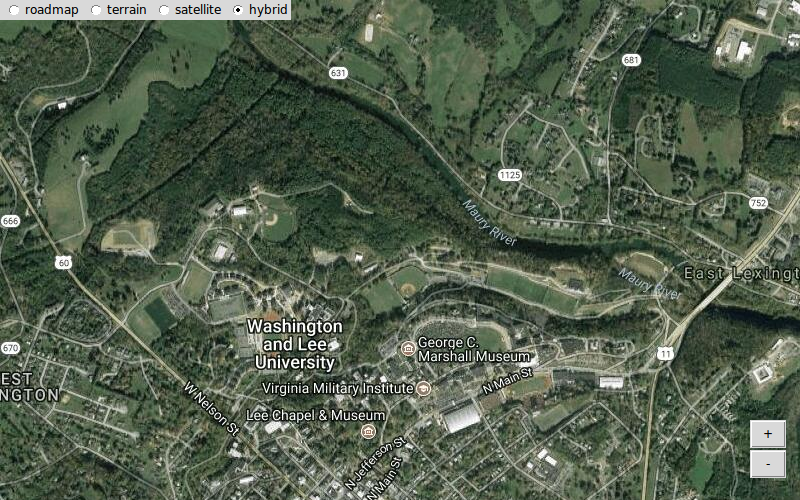
\includegraphics[width=16cm]{goompy}
\centering
\caption{A Goompy implementation of Google's static map API}
\label{fig:the_goompy}
\end{figure}